
\section{Background}
Thoracic surgeries often face challenges of limited visibility due to the narrow space between the ribs. Traditional surgical methods frequently involve partial rib removal to provide surgeons with adequate access and visibility. This invasive approach leads to longer recovery times and increased post-surgery complications.

The \textbf{Thoracic Camera Project} aims to address these issues by introducing a highly maneuverable thoracic camera system capable of precise actuation and real-time feedback. This system is designed to operate within the chest cavity, providing continuous, clear visualization without the need for rib removal. By combining manual and automatic control, our solution enhances surgical precision, reduces the need for assistants, and promotes minimally invasive procedures.

\section{Technical Descriptions}

\subsection{System Overview}
\subsubsection{Block Diagram}

\paragraph{Level 0}
The Level 0 block diagram, shown in Figure~\ref{fig:level0}, outlines the four primary components of the thoracic camera system: the Camera, Video Processing, Tension Control, and the User Interface. The core functionality of the system revolves around the camera, which is mounted on an actuating platform. This slim and maneuverable camera is inserted into the chest cavity during surgery, providing a live video feed.

\begin{figure}[H]
    \centering
    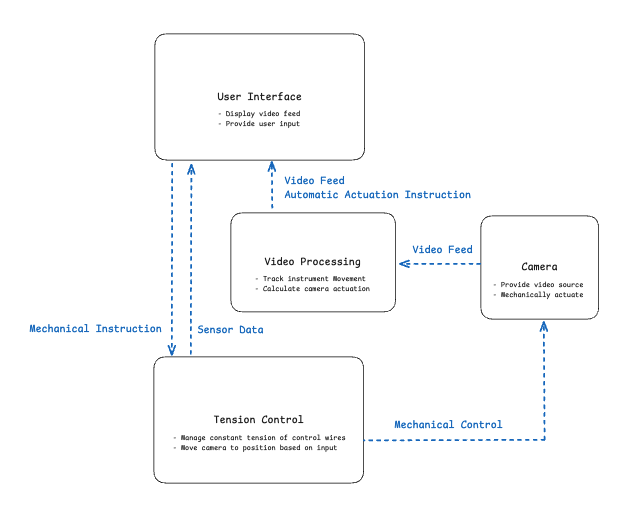
\includegraphics[width=0.8\textwidth]{images/level0.png}
    \caption{Level 0 Block Diagram of the Thoracic Camera System}
    \label{fig:level0}
\end{figure}

The video feed is processed in the Video Processing module, where frames are analyzed to detect surgical tools and calculate the necessary movements to center the object within the frame. These calculated movement commands are forwarded to the Tension Control system, which adjusts the tension in the wires to precisely move and stabilize the camera as needed.

The User Interface (UI) provides surgeons with full control over the system, offering options for both automatic and manual operation modes. Through the UI, users can view the live video feed, monitor system diagnostics, and adjust settings such as brightness or control modes. This integration ensures seamless interaction between the surgeon, the visualization system, and the tension control mechanisms.


\paragraph{Level 1}  
As shown in Figure~\ref{fig:level1}, the Level 1 block diagram details the operational units and their interconnections, emphasizing key components such as the \textbf{Raspberry Pi 5}, \textbf{Pi Pico}, \textbf{ADC Modules}, \textbf{Load Cells}, \textbf{Pi Camera V3 Wide}, \textbf{Stepper Motors}, and \textbf{Stepper Drivers}.

\begin{figure}[H]
    \centering
    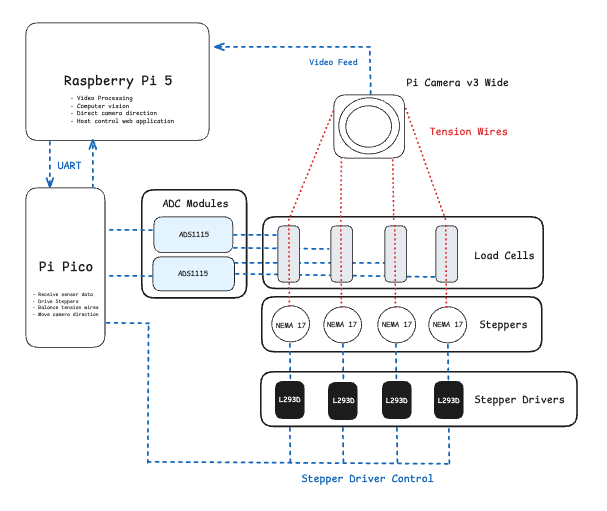
\includegraphics[width=0.8\textwidth]{images/level1.png}
    \caption{Level 1 Block Diagram of the Thoracic Camera System}
    \label{fig:level1}
\end{figure}

\begin{itemize}
    \item \textbf{Pi Camera V3 Wide:} The camera captures high-quality images with a broad field of view, suitable for minimally invasive surgical environments. Its compact design ensures it can navigate tight spaces while providing clear visualization of the surgical field.

    \item \textbf{Raspberry Pi 5:} Serving as the central processing unit, the Raspberry Pi 5 handles computer vision tasks, detecting and tracking objects in the camera feed. It calculates movement adjustments to keep targets aligned at the frame center and hosts the web-based User Interface for real-time video streaming, diagnostics, and control options.

    \item \textbf{Pi Pico:} The Raspberry Pi Pico manages mechanical actuation by controlling four \textbf{Stepper Motors} via \textbf{L293D Stepper Drivers}. It adjusts the tension in four wires attached to the camera mount to ensure smooth movement. The Pico also processes sensor data from the \textbf{ADC Modules} and dynamically balances wire tension to stabilize the camera.

    \item \textbf{ADC Modules:} Two ADS1115 ADC modules interface with the system's \textbf{Load Cells}, reading tension data to ensure precise control. These modules enable continuous monitoring of wire tension and provide feedback for real-time adjustments.

    \item \textbf{Load Cells:} Four load cells measure the tension in each wire, providing critical data to the Raspberry Pi Pico. This feedback allows the system to dynamically adjust wire tension and maintain stability during movement.

    \item \textbf{Stepper Motors:} Four NEMA 17 stepper motors provide the mechanical actuation required to adjust wire tension and position the camera. These motors are controlled by the Raspberry Pi Pico through the \textbf{Stepper Drivers}.

    \item \textbf{Stepper Drivers:} Four L293D drivers serve as the interface between the Raspberry Pi Pico and the stepper motors, enabling precise control over the camera's position and orientation through wire tension adjustments.
\end{itemize}

The integration of these components ensures smooth, responsive, and precise camera movements. The \textbf{Raspberry Pi 5} and \textbf{Pi Pico} communicate via a UART connection, allowing for continuous feedback and command transmission. This seamless interaction between hardware and software provides surgeons with a reliable, intuitive visualization tool for thoracic surgeries, adaptable for both manual and automatic modes.




\subsection{Physical Design}
\subsubsection{Tension Control Module}
The tension control module is responsible for accurately adjusting the position and orientation of the thoracic camera by controlling the tension in four wires connected to the camera. Each module is equipped with a NEMA 17 stepper motor, located at the bottom of the unit, which drives a spool to regulate the tension in the wire. This setup allows for precise control of the camera's movement, crucial for the dynamic visualization required in thoracic surgeries.

For tension monitoring, each module uses a 1kg load cell, which is centrally positioned in the module to measure the exact force applied to the wire. The load cell’s accuracy is key to ensuring balanced tension across all four wires, preventing any misalignment or jerking motions that could interfere with the camera’s positioning. The chosen load cell has an accuracy of ±0.01kg, providing a resolution fine enough to detect even the smallest changes in wire tension. This ensures the camera’s movements are smooth and responsive, which is critical during delicate surgical procedures. 

In terms of physical size, the tension control module, as shown in the attached schematic, is compact yet robust. The overall dimensions are approximately 12.7mm wide by 80mm tall, with a depth of 12.7mm. The wire feeds out from the top of the module through a guiding tube, ensuring that the wire moves smoothly as tension is adjusted. This small form factor makes the system suitable for tight surgical environments, where space is a premium, while still providing the necessary functionality to support the thoracic camera.

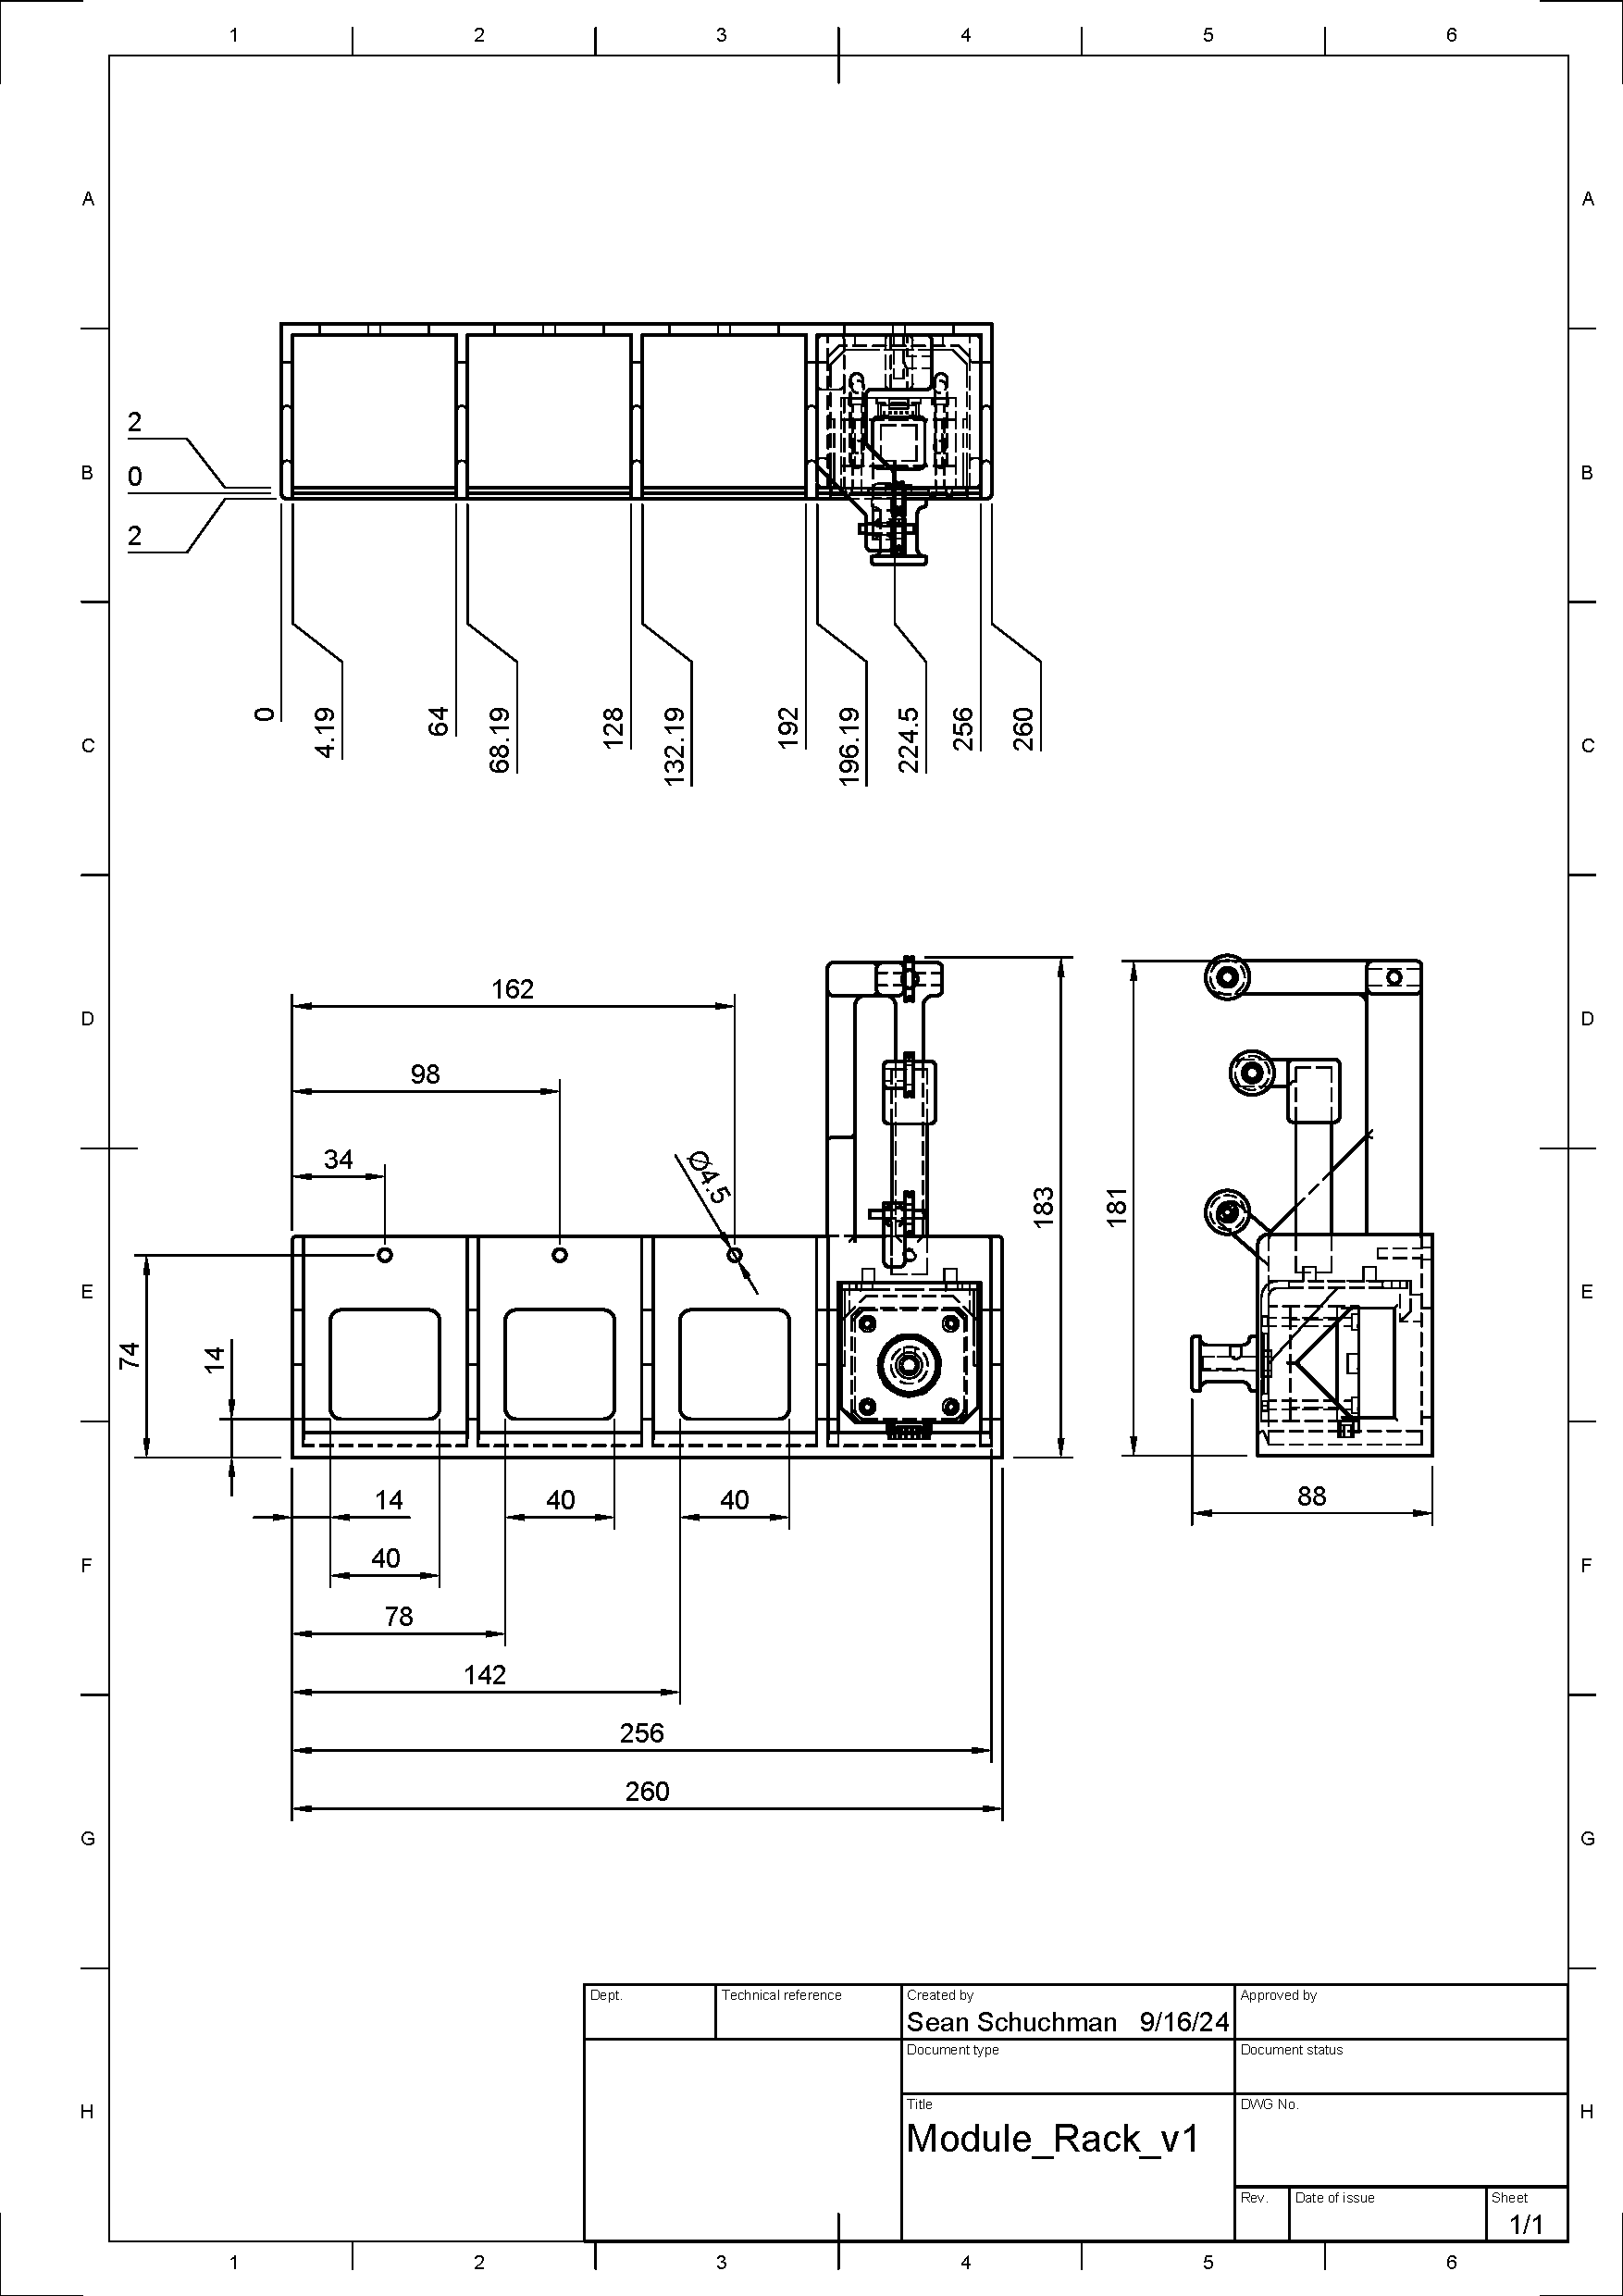
\includepdf[pages=-]{docs/Module_Rack.pdf}

\subsection{Tension Module Rack}
The tension module rack is designed to hold and align the four tension control modules, ensuring they function precisely and consistently during operation. Each module is mounted within the rack, and the rack's dimensions and construction are carefully optimized for stability and ease of assembly. 

The overall length of the rack is 260mm, with a height of 74mm and a depth of 88mm. The modules are spaced 64mm apart, with a set screw positioned at the back of each module, securing them firmly in place. This design prevents any unwanted movement or vibrations, ensuring that the tensioning system remains stable, even under varying loads. The precision alignment of the modules is essential to achieving consistent wire tension and smooth actuation of the thoracic camera. 

Additionally, the rack allows for easy access to each module's stepper motor and load cell for maintenance or adjustment. The rack's design is modular, meaning it can accommodate different configurations or upgrades if needed. This flexibility is critical in surgical environments, where equipment must be adaptable and reliable. 

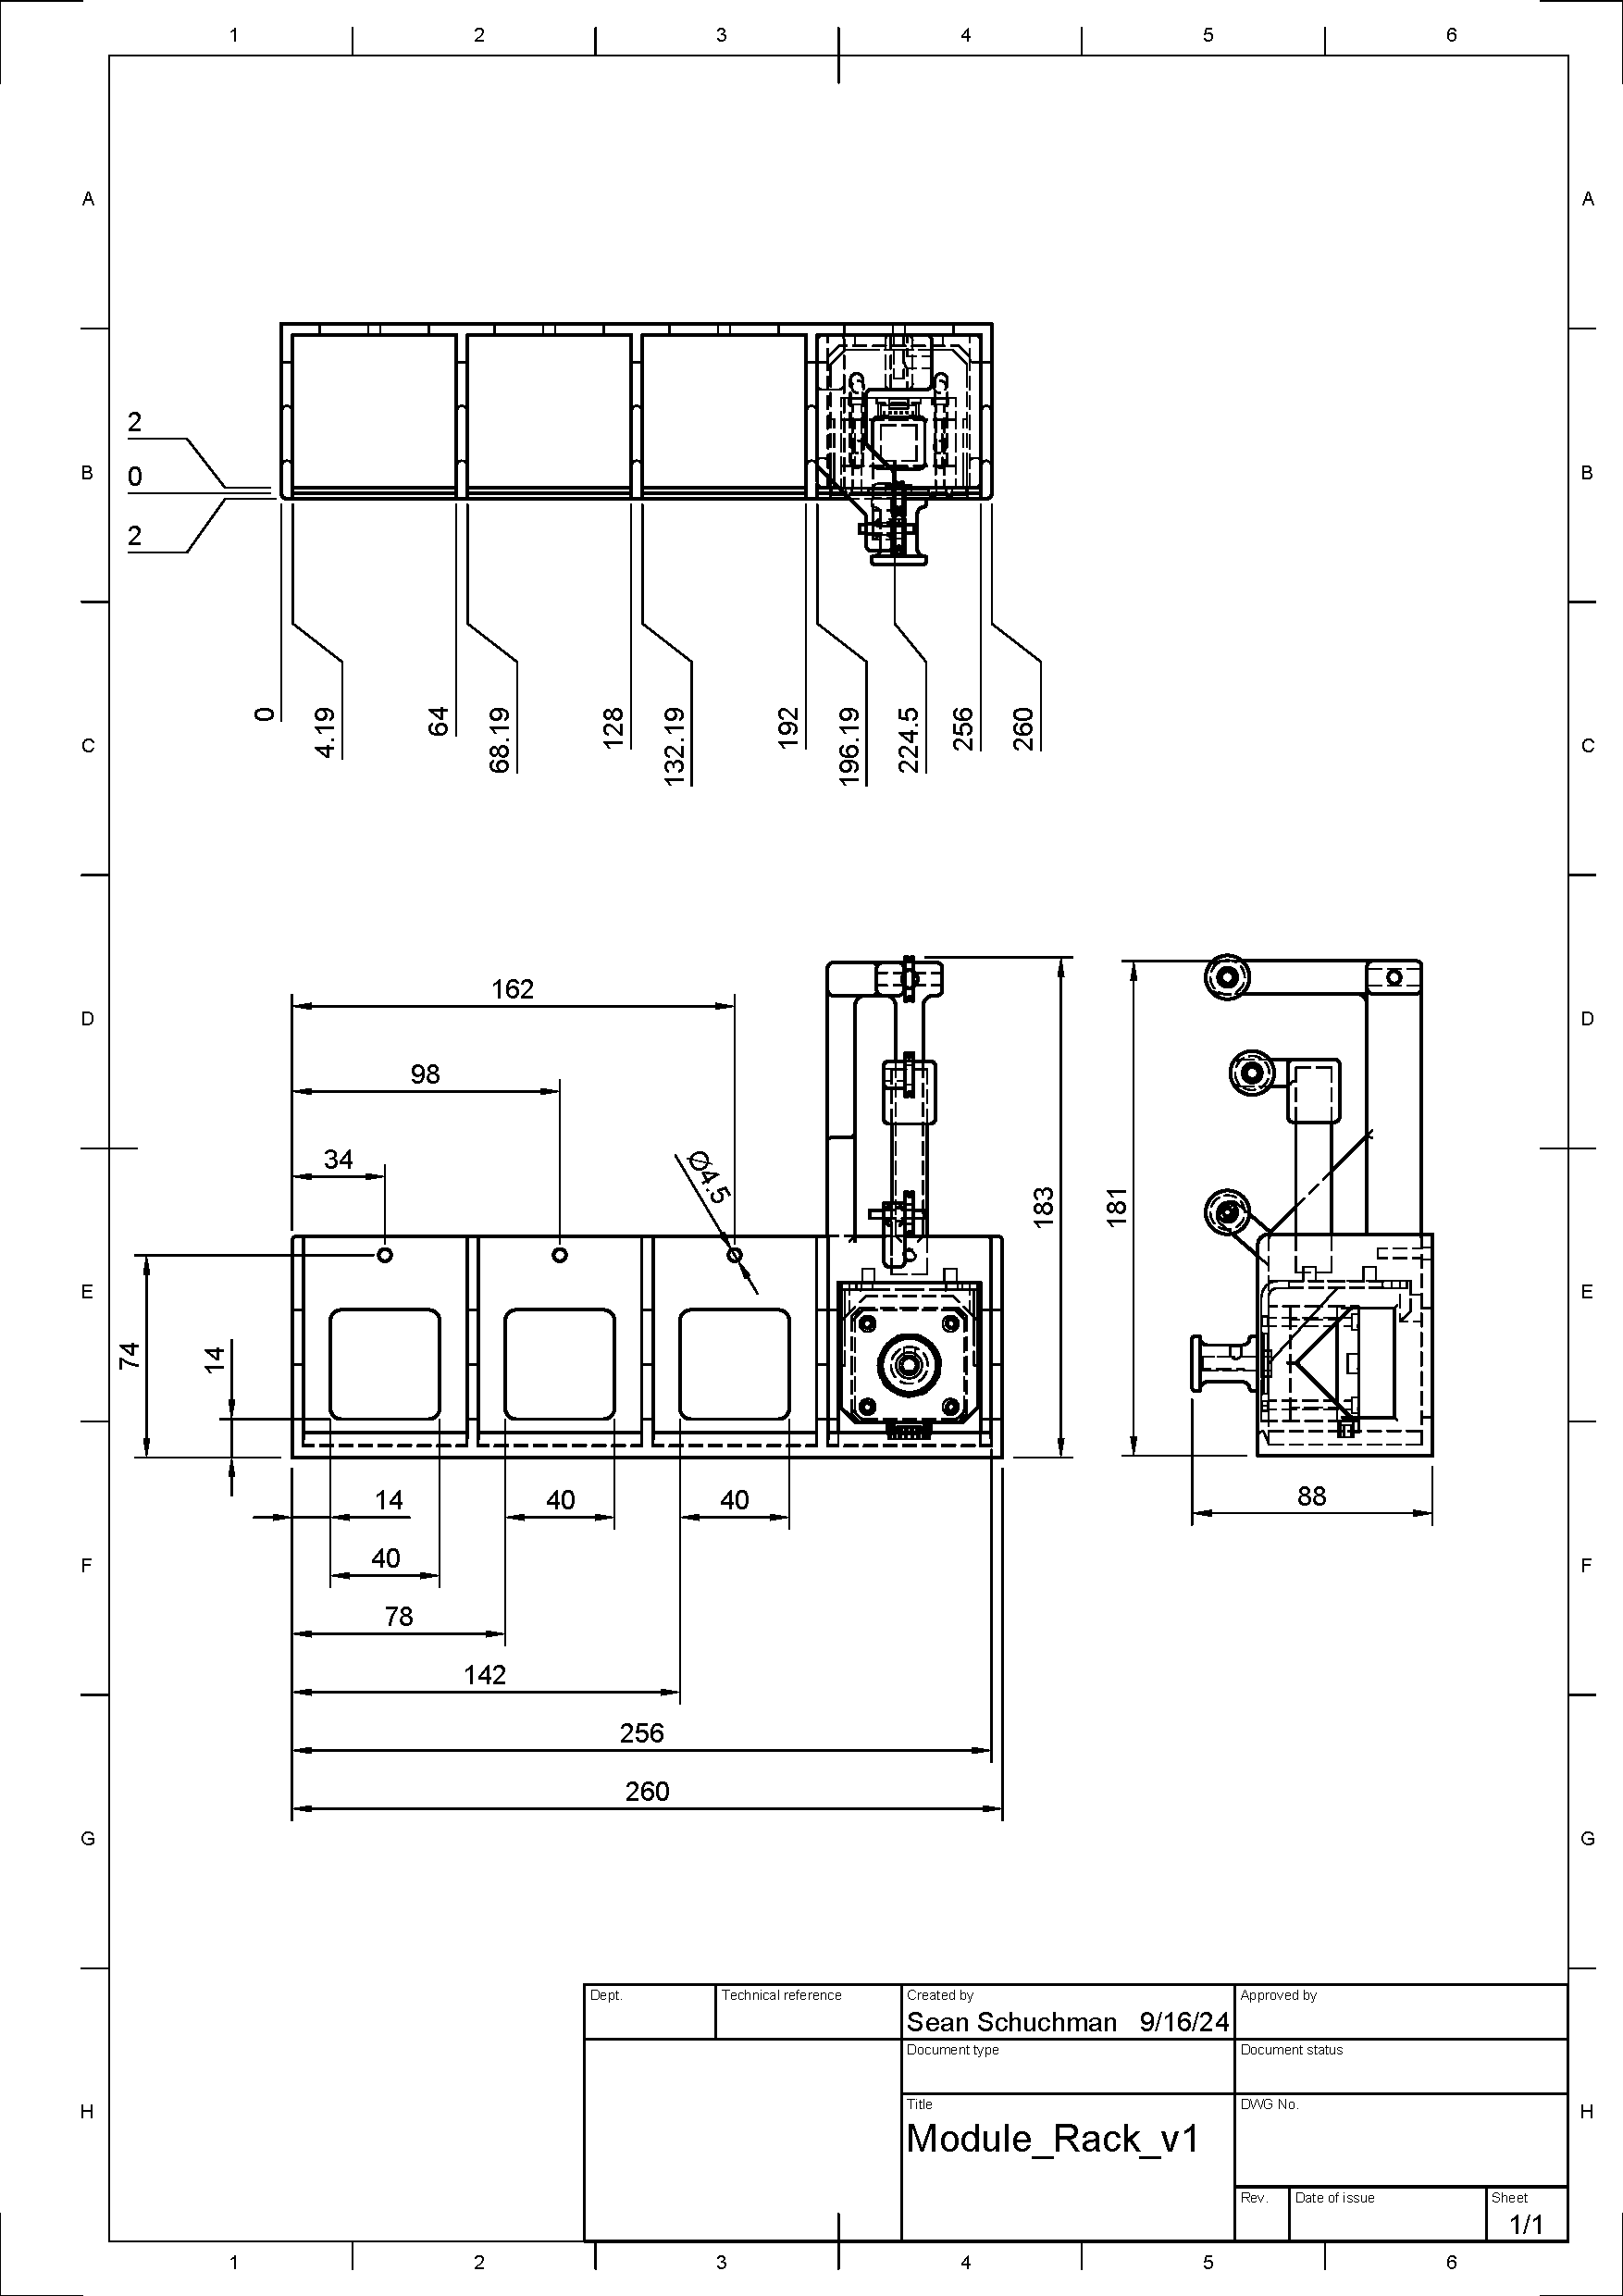
\includepdf[pages=-]{docs/Module_Rack.pdf}

\subsubsection{Camera Module}
\begin{itemize}
    \item Mounted on a gimbal plate actuated by four tension wires for precise directional control.
    \item Includes optimized internal tunnels to reduce friction and enhance movement responsiveness.
    \item Dimensions: 40mm wide, 60mm long, and slightly taller than 15.75mm.
\end{itemize}

The camera module consists of two key components: the platform and the gimbal plate. The platform secures the tension wires, each routed through dedicated tubes and locked into place using set screws. These tubes ensure that the tension wires remain aligned as they apply force to the gimbal plate for movement control. The set screws provide a firm grip on the wires, preventing any slippage, which is critical for maintaining precise camera movement. 

Mounted on a central pedestal, the gimbal plate holds the camera and allows for precise directional control in response to tension adjustments. The tension wires are connected at each corner of the gimbal plate, creating a balanced system that ensures smooth and accurate movement in all directions. 

An iteration of this design introduces an optimized internal tunnel within the base of the camera mount. This adjustment reduces the number of sharp turns that the tension wires must navigate, lowering friction and minimizing wire wear. The smoother path improves force transmission from the stepper motors to the gimbal plate, allowing for more responsive and precise camera movement. However, this optimization has slightly increased the overall height of the design compared to previous versions. This trade-off, favoring smoother action over a slightly taller profile, was necessary to enhance the efficiency and dexterity of the camera movement. 

Despite this change, the overall design remains compact, with the camera module measuring 40mm wide, 60mm long, and now slightly taller than the previous 15.75mm height. This small form factor is still ideal for thoracic surgery, minimizing the amount of hardware within the chest cavity and preventing obstruction of the surgeon’s view. 

Additionally, the camera system eliminates the need for external motors or bulky components inside the surgical area, keeping the setup streamlined. The gimbal plate’s actuation is entirely driven by the tension in the wires, which is managed by stepper motors and load cells located outside of the chest cavity, ensuring smooth, precise, and responsive control during the surgery. 

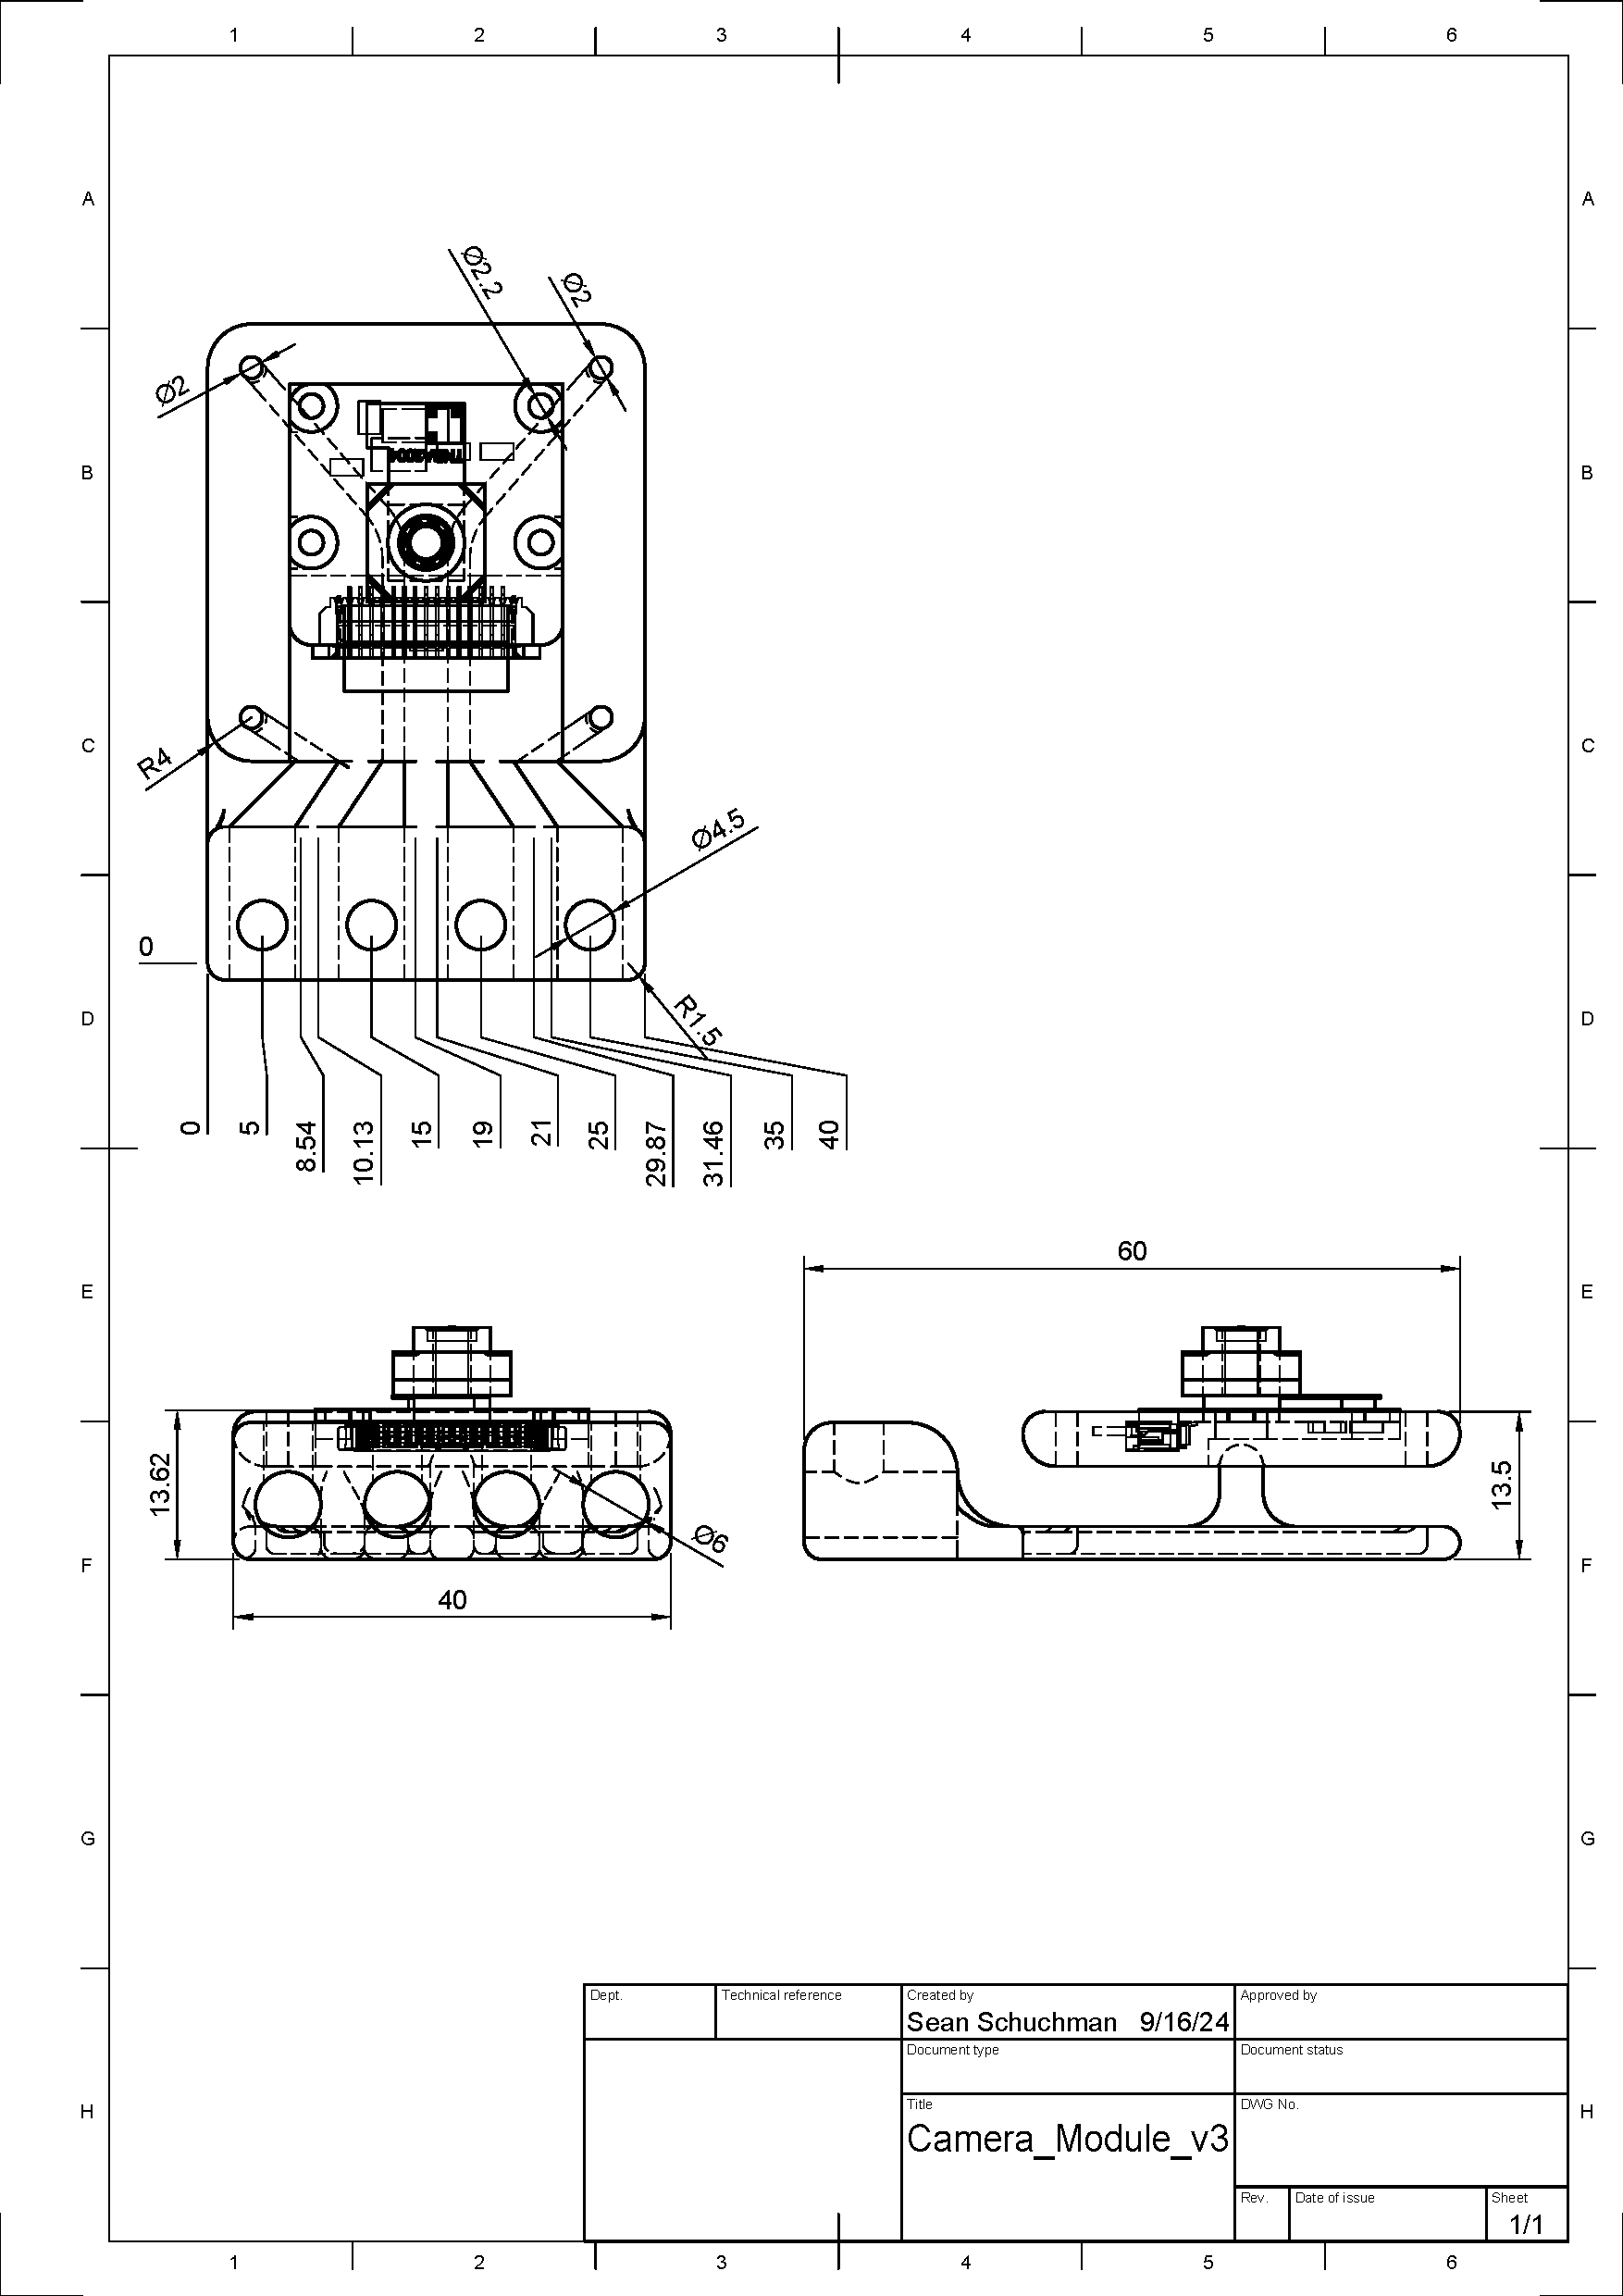
\includepdf[pages=-]{docs/Camera_Module_v3.pdf}

\subsection{Hardware Design}

\subsubsection{Custom PCB Design}

The custom PCB for the thoracic camera system is a crucial component that integrates and organizes all hardware modules for efficient operation. It is designed to accommodate the following features and functionalities:

\begin{itemize}
    \item \textbf{Mounting and Routing:} The PCB includes dedicated mounting holes and routing paths for the \textbf{Raspberry Pi Pico}, \textbf{ADS1115 ADC modules}, and \textbf{L293D Stepper Drivers}. These components are strategically placed to ensure minimal signal interference and efficient power distribution.

    \item \textbf{Debugging Headers:} Debugging headers are provided to facilitate development and troubleshooting. These headers allow seamless access to key signals and communication lines during firmware development and testing.

    \item \textbf{Screw Block Terminals:} Screw block terminals are integrated into the PCB to provide secure connections for external components, including the stepper motors and load cells. These terminals ensure robust mechanical and electrical connections, minimizing the risk of disconnections during operation.

    \item \textbf{24-Pin PC Power Supply Headers:} Female headers are included for compatibility with a standard 24-pin PC power supply. This allows the system to leverage the reliable and high-current output of a PC power supply to drive the motors and other components.

    \item \textbf{Integrated Power Switch:} A power switch is built into the PCB for convenient system control. The switch allows the user to safely power the system on and off without the need to disconnect cables or power supplies.

    \item \textbf{IC Sockets:} IC sockets are used for the stepper drivers and other replaceable components, enabling easy swapping or upgrading without soldering. This feature enhances the maintainability and extendibility of the PCB.

    \item \textbf{Compact and Modular Design:} The PCB design is compact and modular, with clear silkscreen labeling for all connections and components. This ensures that assembly and maintenance can be performed efficiently, even in a high-pressure operating environment.

    \item \textbf{Grounding and Power Distribution:} Proper grounding techniques and wide power traces are used to handle high current demands while minimizing electrical noise. This ensures stable operation of the stepper motors and ADC modules.
\end{itemize}

The PCB not only consolidates the hardware into a single compact unit but also enhances the system's reliability and maintainability. With clearly labeled connections and a well-organized layout, it ensures that all hardware modules can interact seamlessly, supporting the precise and dynamic operation required by the thoracic camera system.

\subsubsection{Raspberry Pi 5}
The Raspberry Pi 5 acts as the central processing unit for the thoracic camera system. It serves several key roles:
\begin{itemize}
    \item \textbf{Computer Vision:} Hosts the OpenCV-based video processing application, which detects and tracks objects within the camera's video feed and calculates movement commands.
    \item \textbf{Web Application:} Runs a Flask-based web application that provides a graphical user interface for live video streaming, manual and automatic control modes, brightness and color range adjustments, and system diagnostics.
    \item \textbf{Communication:} Sends movement commands to the Raspberry Pi Pico and receives sensor data over a UART connection to enable dynamic feedback.
    \item \textbf{Efficient Processing:} Leverages the high-performance quad-core processor to ensure real-time video processing and low-latency system control.
\end{itemize}

\subsubsection{Pi Camera V3 Wide}
The Pi Camera V3 – Wide Angle captures the video feed for the system. Its key attributes include:
\begin{itemize}
    \item \textbf{Wide Field of View:} Provides an extensive view of the surgical field, minimizing blind spots.
    \item \textbf{High Resolution:} Delivers clear, detailed images for precise object detection and tracking.
    \item \textbf{Compact Form Factor:} Enables insertion into tight surgical spaces without obstruction.
\end{itemize}

\subsubsection{Raspberry Pi Pico}
The Raspberry Pi Pico functions as the dedicated hardware controller for the system, responsible for:
\begin{itemize}
    \item \textbf{Motor Control:} Drives four stepper motors using custom-written firmware and L293D stepper motor drivers to adjust the tension in the wires connected to the camera.
    \item \textbf{Sensor Integration:} Reads analog data from ADS1115 ADC modules connected to load cells, providing real-time tension monitoring.
    \item \textbf{Dynamic Adjustment:} Implements a feedback loop to ensure balanced wire tension during camera movements, maintaining stability and precision.
    \item \textbf{Multicore Processing:} Utilizes the dual-core architecture to manage motor control and sensor data independently, ensuring smooth and efficient operation.
\end{itemize}

\subsubsection{L293D Stepper Drivers}
The L293D motor drivers are used to control the NEMA 17 stepper motors. Key features include:
\begin{itemize}
    \item Dual H-bridge configuration for driving bipolar stepper motors.
    \item Control signals provided by the Raspberry Pi Pico to execute precise stepper motor movements.
    \item Compact design integrated onto the custom PCB for easy installation and replacement.
\end{itemize}

\subsubsection{NEMA 17 Stepper Motors}
The system employs four NEMA 17 stepper motors to actuate the tension wires. These motors offer:
\begin{itemize}
    \item \textbf{High Precision:} Capable of microstepping for smooth and accurate movements.
    \item \textbf{Compact Size:} Suitable for integration into the compact tension control module design.
    \item \textbf{Reliable Operation:} Provides consistent performance under variable loads.
\end{itemize}

\subsubsection{ADS1115 ADC Modules}
The ADS1115 ADC modules interface with the load cells to provide high-precision tension data. Features include:
\begin{itemize}
    \item \textbf{Differential Measurements:} Capable of measuring the voltage difference across the load cell's Wheatstone bridge.
    \item \textbf{I2C Communication:} Reduces the number of GPIO pins required for integration with the Raspberry Pi Pico.
    \item \textbf{High Resolution:} Provides 16-bit analog-to-digital conversion for accurate tension readings.
\end{itemize}

\subsubsection{Load Cells}
The load cells provide critical feedback on the tension applied to the wires. Features include:
\begin{itemize}
    \item \textbf{1kg Load Capacity:} Ensures accurate tension monitoring within the system's operational range.
    \item \textbf{High Precision:} Connected to ADS1115 ADC modules to measure minute changes in tension.
    \item \textbf{Robust Design:} Mounted securely on the custom PCB to minimize noise and maintain stability.
\end{itemize}


This hardware design, with its carefully selected components and custom PCB, ensures the system operates reliably and efficiently under the demands of thoracic surgery. Each module is integrated seamlessly to provide surgeons with precise control and a clear visualization of the surgical field.

\subsection{Firmware and Software Design}

The firmware and software design work in unison to deliver a seamless and efficient control system for the thoracic camera. Both the firmware running on the Raspberry Pi Pico and the software hosted on the Raspberry Pi 5 are tailored to achieve precise camera control, real-time feedback, and user interaction. The integration of these two components enables the system to provide reliable performance under the demands of surgical applications. The high-level architecture of this integration is illustrated in Figure~\ref{fig:software_flowchart}.

\begin{figure}[H]
    \centering
    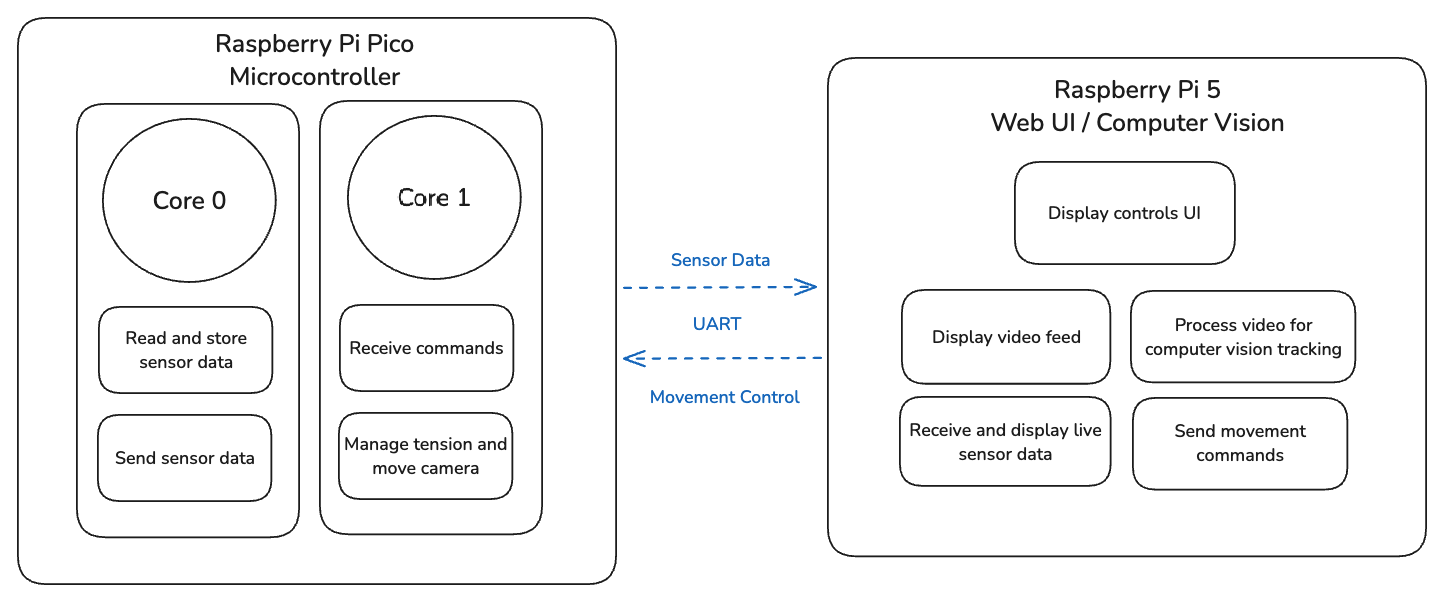
\includegraphics[width=0.8\textwidth]{images/software_flowchart.png}
    \caption{Firmware and Software Flowchart}
    \label{fig:software_flowchart}
\end{figure}


\subsubsection{Firmware Design}
The firmware for the thoracic camera system was meticulously crafted to provide precise control of the stepper motors and accurate monitoring of load cell data, enabling real-time actuation of the camera module. Written in C, the firmware leverages the full capabilities of the Raspberry Pi Pico, including its dual-core processor, to optimize performance and responsiveness. Custom drivers were developed from scratch for critical components such as the L293D motor drivers, ADS1115 analog-to-digital converters (ADCs), and UART communication, ensuring full control and flexibility over the hardware.

Core 0 of the Raspberry Pi Pico is dedicated to high-priority tasks such as receiving commands from the Raspberry Pi 5 via UART and executing motor control routines. The UART communication interface continuously listens for movement commands in the form of Move[x, y], where x and y dictate the directional control of the camera. These commands are parsed and validated before the motors are activated. The movement routines adjust wire tension by stepping the corresponding motors either forward or backward based on load cell feedback, ensuring precise and balanced actuation. The motor drivers use custom microstepping sequences implemented in the firmware to provide smooth and accurate movements.

Core 1 is responsible for monitoring the load cell data by interfacing with two ADS1115 ADC modules configured in differential mode. Each ADC monitors two load cells, allowing the system to measure the tension in all four wires simultaneously. The ADS1115 driver was custom-built to initialize the ADCs, perform calibration, and retrieve differential voltage readings at a high sampling rate. These readings are processed and stored in a shared data structure, protected by mutexes to prevent race conditions. This modular design ensures that load cell data is continuously updated without interrupting the real-time responsiveness of motor control operations on Core 0.

The firmware's calibration routine ensures the system is correctly aligned before operation. During calibration, each stepper motor unwinds the tension wires to a safe baseline, while the ADS1115 modules measure and offset any discrepancies in the load cell readings. Once the baseline tension is set, the motors are activated to bring the wires to their optimal tension range, guaranteeing smooth and precise movements during operation.

The firmware also incorporates safeguards and intelligent error handling. For example, the motor control routines actively monitor the tension limits using load cell data to prevent over-tightening or slack in the wires. If the tension exceeds the predefined upper or lower thresholds, the firmware stops the motors and adjusts as necessary to maintain balance.

By utilizing the Pico's dual-core architecture, the firmware efficiently separates computational tasks, ensuring that motor control and load cell monitoring run concurrently and without interference. This design enables seamless coordination between the hardware components and the software system, allowing for precise real-time adjustments required during minimally invasive thoracic surgeries. The custom-built drivers and modular firmware structure provide a reliable and extensible foundation for future enhancements and adaptability to additional hardware components.

For further details and to reference the implementation, please visit the GitHub repository at \url{https://github.com/sschuchman/thorCam}. Specifically, navigate to the \texttt{/Firmware/thorCam} directory for access to the software codebase.

\subsubsection{Software Design}
The software design of the thoracic camera system integrates multiple components to provide real-time control and visualization. At the core of the system, an OpenCV-based program running on the Raspberry Pi 5 handles object detection. This program processes the live video feed to identify objects based on their color and calculates their offset from the center of the frame. Using this information, movement commands are generated and sent to the Raspberry Pi Pico via a Flask-based server. The Pico receives these commands over UART and drives the stepper motors to adjust the camera's position, enabling real-time, smooth actuation. In automatic mode, the camera continuously tracks the object and adjusts its position to keep the object centered in the frame without requiring user input.

The user interface, implemented as a web application using Flask, provides seamless interaction between the operator and the system. It supports both manual and automatic control modes. In manual mode, users can operate the camera using on-screen directional buttons or keyboard keys, while in automatic mode, the system autonomously tracks the object and adjusts the camera position accordingly. The interface also features a live video feed for real-time visualization, a mask feed that highlights the detected object with bounding boxes and offset lines, and a dynamic bar chart displaying tension data from the load cell sensors. Additional interface features include sliders for adjusting brightness and HSV color thresholds, as well as toggle switches for selecting control modes and activating a demo mode.

To ensure optimal system performance, the software processes the video feed at 1920x1080 resolution, overlaying critical information such as bounding boxes, offsets (\textit{dx} and \textit{dy}), and object distances. A separate thread continuously monitors the UART connection to receive and log tension data from the load cells, which is displayed in the web application in real time. The mask feed uses HSV-based filtering and contour analysis to visualize the object detection process, aiding in debugging and parameter optimization.

The software is designed to provide a flexible and responsive user experience, allowing the operator to configure system parameters dynamically. Users can fine-tune brightness and color thresholds through the web interface to adapt to changing lighting conditions. The demo mode automates pre-defined movement patterns for testing and demonstration purposes. These capabilities, combined with seamless integration between the Raspberry Pi 5 and Pico, ensure precise and efficient control of the thoracic camera system.

For further details and to reference the implementation, please visit the GitHub repository at \url{https://github.com/sschuchman/thorCam}. Specifically, navigate to the \texttt{/Software/thor-controller} directory for access to the software codebase.

\subsection{System Performance}
The thoracic camera system delivers real-time responsiveness and precision through the integration of efficient firmware and software, tailored for minimally invasive surgical applications.

On the firmware side, the Raspberry Pi Pico leverages its dual-core architecture to handle sensor data acquisition and motor control independently. Core 1 manages load cell readings from two ADS1115 ADCs in differential mode, updating all four tension values approximately every 10 milliseconds. Core 0 handles stepper motor control and UART communication, with motor movements executed in 10–15 microseconds per microstep. Typical movement commands, involving both sensor feedback and tension adjustments, are processed within 50–100 milliseconds, ensuring smooth, dynamic actuation.

The software on the Raspberry Pi 5 integrates video processing, user interface, and communication with the firmware. OpenCV-based object tracking processes frames at 30 FPS (33 ms per frame), calculating offsets and sending movement commands with a transmission latency of less than 20 milliseconds. The Flask web interface refreshes live video and mask feeds at 30 FPS, while tension sensor data is updated every 100 milliseconds, providing a responsive and intuitive user experience.

Together, the system achieves near-instantaneous feedback and control with key performance benchmarks: sensor updates at 100 Hz, stepper command execution in under 100 milliseconds, and real-time UI updates. These metrics ensure the system's reliability, making it ideal for delicate surgical procedures requiring precision and minimal latency.

\begin{itemize}
    \item \textbf{Sensor Update Rate:} 100 Hz (every 10 ms)
    \item \textbf{Stepper Command Execution:} $~$50–100 ms
    \item \textbf{Video Feed and Mask Refresh Rate:} 15 FPS (software limited to 30 FPS)
    \item \textbf{Sensor Data Display Refresh Rate:} 10 Hz (every 100 ms)
    \item \textbf{Transmission Latency:} $<$20 ms
\end{itemize}

\section{Final Schedule}
\begin{tabular}{|l|l|l|}
    \hline
    Task & Responsible Party & Completion Date \\ \hline
    Physical Design Prototyping & All Contributors & September 2024 \\ \hline
    Hardware Assembly & Jakob Schoeberle & October 2024 \\ \hline
    Software Development & Sean Schuchman & November 2024 \\ \hline
    System Integration and Testing & All Contributors & December 2024 \\ \hline
\end{tabular}

\section{Distribution of Effort}
\begin{tabular}{|l|l|}
    \hline
    Contributor & Area of Contribution \\ \hline
    Sean Schuchman & 3D Modeling, Manufacturing, Software/Firmware Design, Prototyping \\ \hline
    Jakob Schoeberle & Circuit Design, PCB Design, PCB Assembly \\ \hline
    Colton Wall & Research, Hardware Assembly, System Integration \\ \hline
\end{tabular}

\section{Possible Future Work}
The thoracic camera system has demonstrated its potential as a reliable surgical visualization tool, but several areas of improvement can be pursued to enhance its functionality, usability, and application scope:

\begin{itemize}
    \item \textbf{Miniaturization and Physical Redesign:} Scale down the size of the camera probe and tension control module to make the system less intrusive and more versatile for broader surgical applications. A redesigned camera platform can improve maneuverability in confined spaces.

    \item \textbf{Integrated Lighting and Compact PCB:} Develop a custom PCB with integrated LED lighting for the camera, minimizing the system's footprint and reducing the need for additional external components.

    \item \textbf{PID Control for Camera Movement:} Replace the heuristic-based movement algorithm with a PID (Proportional-Integral-Derivative) control system. This would provide more precise, stable, and responsive control over camera movements.

    \item \textbf{Alternative Control Options:} Explore wireless control systems to eliminate the need for physical cabling in the operating room or integrate foot pedal controls to give surgeons hands-free operation.

    \item \textbf{Medical-Grade Material Design:} Transition to medical-grade materials for the camera probe, tension wires, and platform to ensure biocompatibility, sterilizability, and compliance with healthcare regulations.

    \item \textbf{AI-Based Object Tracking:} Implement AI-based object detection and tracking algorithms to improve the accuracy, robustness, and response time of the system's automatic mode.

    \item \textbf{System Robustness and Durability:} Enhance the durability of tension wires, load-bearing components, and the gimbal plate to withstand repeated use in clinical environments without performance degradation.

    \item \textbf{Clinical Trials and Validation:} Conduct extensive testing in simulated and real surgical environments to validate the system's reliability, safety, and usability in various medical procedures.
\end{itemize}

These advancements would not only improve the overall functionality and performance of the system but also increase its adaptability for diverse surgical applications, bringing it closer to practical deployment in clinical settings.


\section{Conclusion}
The \textbf{Thoracic Camera Project} successfully demonstrates a novel solution for improving visibility and precision in thoracic surgeries. By leveraging advanced hardware and software integration, the system offers a minimally invasive alternative to traditional methods. While challenges remain in miniaturization and clinical testing, the project's results showcase the potential for transformative improvements in surgical outcomes.

\vspace{0.5cm}
\noindent
\textbf{\normalsize For a demonstration of the system, watch the} \href{https://youtu.be/UekYdXSXzXo}{\textbf{\normalsize demo video}}.
\vspace{0.5cm}



\subsection{References}
\begin{itemize}
    \item Raspberry Pi Documentation: \url{https://datasheets.raspberrypi.com/rpi5/raspberry-pi-5-product-brief.pdf}
    \item Raspberry Pi Pico Documentation: \url{https://datasheets.raspberrypi.com/pico/pico-datasheet.pdf}
    \item Raspberry Pi Pico C/C++ SDK: \url{https://www.raspberrypi.com/documentation/microcontrollers/c_sdk.html}
    \item OpenCV Python Documentation: \url{https://opencv.org}
    \item NEMA 17 Datasheet: \url{https://pages.pbclinear.com/rs/909-BFY-775/images/Data-Sheet-Stepper-Motor-Support.pdf}
    \item L293D Motor Driver Datasheet: \url{https://www.ti.com/product/L293D}
    \item ADS1115 ADC Datasheet: \url{https://www.ti.com/lit/ds/symlink/ads1115.pdf}
\end{itemize}

\section{Bill of Materials}

\begin{tabular}{|l|l|c|c|c|c|}
    \hline
    \textbf{Name} & \textbf{Description} & \textbf{Quantity} & \textbf{Price (USD)} & \textbf{Cost (USD)} & \textbf{Link} \\ \hline
    Raspberry Pi 5 & 8GB & 1 & 79.99 & 79.99 & \href{https://www.microcenter.com/product/673711/raspberry-pi-5-8gb-lpddr4x}{Link} \\ \hline
    Pi Pico & Non-wireless & 1 & 3.99 & 3.99 & \href{https://www.microcenter.com/product/661033/raspberry-pi-pico-microcontroller-development-board}{Link} \\ \hline
    L293D & Stepper Motor Driver (10 pcs) & 1 & 8.99 & 3.60 & \href{https://www.amazon.com/gp/product/B09NBQYVLL/ref=ppx_yo_dt_b_asin_title_o00_s00}{Link} \\ \hline
    M3 Screw Set & Metric Screws with Nuts & 1 & 8.99 & 1.18 & \href{https://www.amazon.com/dp/B0BMQFHD8H?ref_=yo_ov_dt_b_fed_asin_title}{Link} \\ \hline
    Ball Bearing & 3mm Bore & 1 & 8.29 & 4.97 & \href{https://www.amazon.com/dp/B07WF18HQY?ref_=ppx_yo2ov_dt_b_fed_asin_title}{Link} \\ \hline
    Threaded Inserts & M3 brass threaded insert & 1 & 6.99 & 2.10 & \href{https://www.amazon.com/dp/B0CCX33LHD?ref_=ppx_yo2ov_dt_b_fed_asin_title}{Link} \\ \hline
    Mount Bracket & Nema 17 mounting bracket (4 pcs) & 1 & 14.99 & 14.99 & \href{https://www.amazon.com/dp/B07JW6X9ZR?ref_=ppx_yo2ov_dt_b_fed_asin_title}{Link} \\ \hline
    Load Cell & 1kg load cell (4 pcs) & 1 & 15.49 & 15.49 & \href{https://www.amazon.com/dp/B09YTQKQ9G/ref=ppx_yo_dt_b_search_asin_title}{Link} \\ \hline
    Pi Camera & Pi Camera V3 – Wide & 1 & 34.99 & 34.99 & \href{https://www.microcenter.com/product/662018/raspberry-pi-camera-3-wide}{Link} \\ \hline
    Camera Cable & Standard $\rightarrow$ Mini Pi camera cable & 1 & 1.99 & 1.99 & \href{https://www.microcenter.com/product/671933/raspberry-pi-5-camera-cable-300mm}{Link} \\ \hline
    Printed Circuit Board & Custom Designed PCB & 5 & 60.92 & 60.92 & \href{https://jlcpcb.com/}{Link} \\ \hline
    PCB Components & Electrical Components & n/a & 22.75 & 22.75 & \href{https://www.digikey.com/}{Link}\\ \hline
    \textbf{Total} &  &  & \textbf{268.37} & \textbf{247.96} &  \\ \hline
\end{tabular}


\section{Acknowledgements}
We extend our gratitude to:
\begin{itemize}
    \item \textbf{Dr. Amardeep Kaur} for her guidance and mentorship throughout the project.
    \item \textbf{Dr. Timothy York} for technical specifications and project requirements.
    \item \textbf{Craig Watson} for technical guidance and perspective throughout the project.
    \item \textbf{SIUE (Southern Illinois University Edwardsville) URCA (Undergraduate Research and Creative Activities)} for allowing us to adopt the Thoracic Camera Project as a senior design project.
    \item \textbf{SIUE ECE (Electrical and Computer Engineering) Department} for providing the resources and lab space.
\end{itemize}
